\chapter{Spielkonzepte}

{\color{red}Benötigte Technische Lösungen jeweils nennen}

Einige Hilfsmittel, die zur Umsetzung der oben genannten Beispiel-Spiele notwendig oder
hilfreich sind.

Um die oben genannten Spiele um einen virtuellen Teil erweitern zu k�nnen werden Konzepte ben�tigt. Eine von uns getroffene Auswahl wird im folgenden beschrieben. 

\section{Erweiterte Realit�t}
Konzepte, die explizit die Realit�t erweitern und dadurch einen Mehrwert zum Spiel beitragen.


\subsubsection{Integration virtueller Objekte in die physische Umgebung}\label{sec:integration-virtueller-objekte-in-die-physische-umgebung}
Um ein virtuelles Spiel in die physische Umgebung integrieren zu k�nnen, m�ssen auch alle Objekte des virtuellen Spieles in die physische Umgebung gebracht werden. Dies kann z.B. auf einer virtuellen Karte, die die Wirklichkeit widerspiegelt, geschehen.

Zum Beispiel die Items bei unserem Spiel Snake, die es einzusammeln gilt, werden auf einer Karte auf dem Smartphone dargestellt und durch einen eingeschr�nkten Zufall platziert. Bei dem ein oder anderen Spiel soll es eine Basis f�r jedes Team geben. Dabei bietet sich an, dieses auf eine relativ freie Fl�che festzusetzen. Generell sollte darauf geachtet werden, dass die Objekte nicht innerhalb eines Geb�udes landen oder in nicht begehbares/erreichbares Terrain platziert werden.



Dies kann mit Hilfe der folgenden technischen L�sungen umgesetzt werden. Die Kartendarstellung (s. \ref{kartendarstellung}) hilft enorm die Objekte in die physische Welt einzuarbeiten, da sie lediglich auf der Karte eingef�gt werden m�ssen. Mit der Kollisionsabfrage (s. \ref{kollisionsabfrage}) kann eine Kollision zweier Objekte, zum Beispiel eine "`Snake"' mit einem "`Item"', verwirklicht werden. Die Positionsabfrage wird unter anderem daf�r ben�tigt um sicherzustellen, dass das Objekt in der N�he des Spielers erstellt wird. (s. \ref{positionsermittlung}).

\subsubsection{Darstellung der physischen und virtuellen Umgebung}\label{sec:darstellung-der-physischen-und-virtuellen-umgebung}

Die physische Welt in eine virtuelle Umgebung zu �bertragen kann einen enormen Mehrwert des Spiels darstellen.
Sei es in einer Karte als �bersicht oder lediglich eine Anzeige ob man sich innerhalb bzw. au�erhalb des Spielfelds befindet. Des weiteren kann mit den heutigen Smartphones auch wie in  Abbildung \ref{fig:aug01} gezeigt eine Augmented Reality geschaffen werden, die die Darstellung der realen Welt um etwa die Beschriftung der zu sehenden Gesch�fte erweitert.
\begin{figure}[htbp]
  \centering
    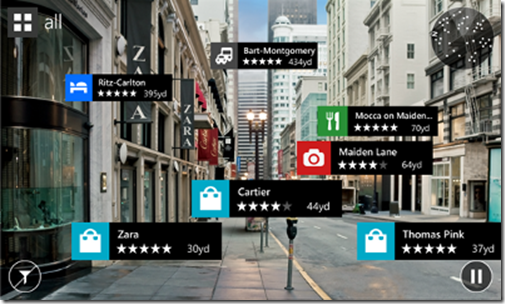
\includegraphics[width=0.9\textwidth]{3-Spielkonzepte/3-1-Erweiterte_Realitaet/map01.png}
    
		\caption{Handyscreen um die zu sehenden Gesch�fte, Hotels, etc. erweitert
	(Quelle: \url{http://blogs.bing.com/maps/wp-content/uploads/sites/3/2013/06/clip_5F00_image006_5F00_thumb_5F00_4AEFDB0C.png})
		}
		\label{fig:aug01} 
\end{figure}
 Hierf�r werden Kartendarstellung (s. \ref{kartendarstellung}) und Positionsermittlung (s. \ref{positionsermittlung}) ben�tigt.

\subsubsection{Kollision virtueller Objekte}\label{sec:kollision-virtueller-objekte}
Treffen zwei virtuelle Objekte aufeinander kann ein Event ausgel�st werden. Wird bei Snake z.B. der eigene Schwanz ber�hrt, was laut der Regeln nicht erlaubt ist, muss dies dem Spieler mitgeteilt werden und evtl. weitere Ereignisse ausgef�hrt werden.

Dazu werden die Kollisionsabfrage (s. \ref{kollisionsabfrage}) und die  Positionsermittlung (s. \ref{positionsermittlung}) gebraucht.


\subsubsection{Einsammeln von Objekten}\label{sec:einsammeln-von-objekten}
Eine Variante der Kollision mit virtuellen Objekten ist das Einsammeln. Wenn ein Spieler in Reichweite eines Items ist, das es einzusammeln gilt, kann dies entweder automatisch passieren oder �ber eine Aufforderung auf dem mobilen Ger�t. Zur Best�tigung, dass etwas eingesammelt wurde, kann nun wiederum ein akustisches oder haptisches Signal gegeben werden.

 Erreicht werden kann dies durch die Positionsermittlung (s. \ref{positionsermittlung}) und die Kollisionsabfrage (s. \ref{kollisionsabfrage}). F�r weitere Best�tigungssignale sind auch andere Sensorik (s. \ref{sensorik}) von Vorteil.


\section{Benutzer Interface}



Konzepte, die haupts�chlich dazu dienen mit dem Spieler zu interagieren und sehr abh�ngig von seinen Entscheidungen sind.


\subsubsection{Kompass}
\begin{wrapfigure}{r}{0.4\textwidth}
  \begin{center}
    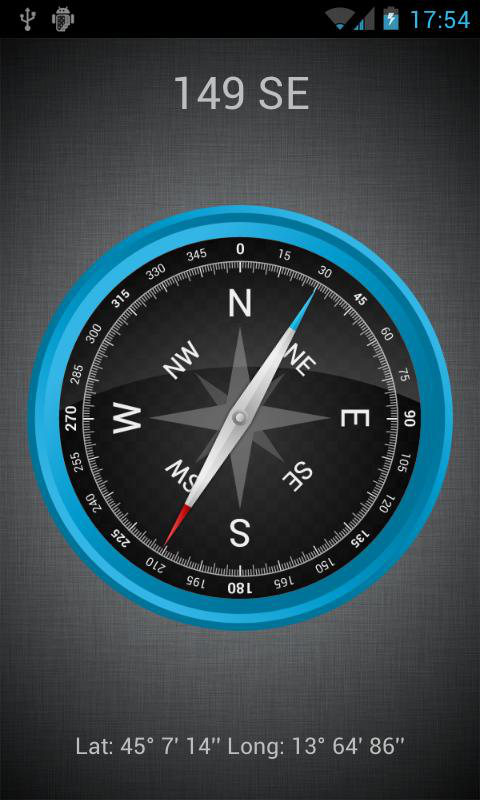
\includegraphics[width=0.3\textwidth]{3-Spielkonzepte/3-2-Benutzer_Interface/kompass.png}
     \caption{integrierter Kompass unter Android}
  \end{center}
\end{wrapfigure}

Eine Richtungsangabe kann eine Karte ersetzen. Sei es um bei �Capture the Flag� die
Richtung der Fahne des Gegners anzuzeigen oder f�r die �Snake� das n�chste
einzusammelnde Item. In der Regel hat es hier weniger Sinn, wenn die Kompassnadel nach
Norden zeigt.
\newline
Technische L�sungen:
Positionsermittlung (s. \ref{positionsermittlung}), GUI (s. \ref{gui}), Andere Sensorik (s. \ref{sensorik})

\subsubsection{Akustische und haptische Orientierungshilfen}

Akustische oder haptische Signale k�nnen ebenso Hinweise geben auf in der N�he
befindliche Interessengebiete (z.B. ert�nen eines Signals oder Vibration bei erreichen eines
bestimmtem Umkreises von einem Item). 
K�nnen aber auch als Best�tigung eingesetzt
werden, wenn z.B. etwas eingesammelt wurde.
\newline
Technische L�sungen:
Kollisionsabfrage (s. \ref{kollisionsabfrage}), Andere Sensorik (s. \ref{sensorik})


\subsubsection{Geschwindigkeitsmessung}
Um das Spielgeschehen besser zu kontrollieren zu k�nnen, kann eine Messung der
Geschwindigkeit von Vorteil sein. M�chten wir z.B. bei Capute the Flag dem Fahnentr�ger
nicht erlauben eine gewissen Geschwindigkeit zu �berschreiten, ist eine
Geschwindigkeitsmessung unabdingbar.
\newline
Technische L�sungen:
Positionsermittlung (s. \ref{positionsermittlung}), Server-Client-Kommunikation (s. \ref{kommunikation}), Andere Sensorik (s. \ref{sensorik})


\subsubsection{Mensch-Maschine-Kommunikation}
Das komplette Spielgeschehen lebt nach der Integrierung von mobilen Endger�ten von der Kommunikation zwischen Mensch und Ger�t. Wird auf dem Endger�t ein Kompass angezeigt, muss der Spieler insofern reagieren, dass er sich in die richtige Richtung dreht.
Wenn er etwas einsammeln m�chte, kann es erforderlich sein, dass ein Button gedr�ckt
wird.
\newline
Technische L�sungen:
GUI (s. \ref{gui}), Kartendarstellung (s. \ref{kartendarstellung})

\section{Kompass}

Eine Richtungsangabe kann eine Karte ersetzen. Sei es um bei �Capture the Flag� die
Richtung der Fahne des Gegners anzuzeigen oder f�r die �Snake� das n�chste
einzusammelnde Item. In der Regel hat es hier weniger Sinn, wenn die Kompassnadel nach
Norden zeigt.
\newline
Technische L�sungen:
Positionsermittlung (s. \ref{positionsermittlung}), GUI (s. \ref{gui}), Andere Sensorik (s. \ref{sensorik})

\section{Arkustische und haptische Orientierungshilfen}

Akustische oder haptische Signale k�nnen ebenso Hinweise geben auf in der N�he
befindliche Interessengebiete (z.B. ert�nen eines Signals oder Vibration bei erreichen eines
bestimmtem Umkreises von einem Item). K�nnen aber auch als Best�tigung eingesetzt
werden, wenn z.B. etwas eingesammelt wurde.
\newline
Technische L�sungen:
Kollisionsabfrage (s. \ref{kollisionsabfrage}), Andere Sensorik (s. \ref{sensorik})

\section{Synchronisation zwischen mobilen Endger�ten}

Und hier wieder einf�gen.

\section{Kollision virtueller Objekte}
Treffen zwei virtuelle Objekte aufeinander muss in der Regel ein Event ausgel�st werden.
Wird bei Snake z.B. der eigene Schwanz ber�hrt, was laut der Regeln nicht erlaubt ist, muss
dies dem Spieler mitgeteilt werden und evtl. weitere Ereignisse ausgef�hrt werden.
\newline
Technische L�sungen:
Kollisionsabfrage (s. \ref{kollisionsabfrage}), Positionsermittlung (s. \ref{positionsermittlung})

\section{Einsammeln von Objekten}
Eine Variante der Kollision mit virtuellen Objekten ist das Einsammeln. Wenn ein Spieler in
Reichweite eines Items ist, das es einzusammeln gilt, kann dies entweder automatisch
passieren oder �ber eine Aufforderung auf dem mobilen Ger�t. Zur Best�tigung, dass
etwas eingesammelt wurde, kann nun wiederum ein akustisches oder haptisches Signal
gegeben werden.

\section{Geschwindigkeitsmessung}
Um das Spielgeschehen besser zu kontrollieren zu k�nnen, kann eine Messung der
Geschwindigkeit von Vorteil sein. M�chten wir z.B. bei Capute the Flag dem Fahnentr�ger
nicht erlauben eine gewissen Geschwindigkeit zu �berschreiten, ist eine
Geschwindigkeitsmessung unabdingbar.
\newline
Technische L�sungen:
{\color{red}add Links zu}
Positionsermittlung, Server-Client-Kommunikation, Andere Sensorik

\section{Mensch-Maschine-Kommunikation}
Das komplette Spielgeschehen lebt nach der Integrierung von mobilen Endger�ten von der Kommunikation zwischen Mensch und Ger�t. Wird auf dem Endger�t ein Kompass angezeigt, muss der Spieler insofern reagieren, dass er sich in die richtige Richtung dreht.
Wenn er etwas einsammeln m�chte, kann es erforderlich sein, dass ein Button gedr�ckt
wird.
\newline
Technische L�sungen:
GUI (s. \ref{gui}), Kartendarstellung (s. \ref{kartendarstellung}), Andere Sensorik (s. \ref{sensorik})

\section{Chat}
Um mit seinen Teammitgliedern oder dem gegnerischen Team zu kommunizieren gibt es
eine Reihe von M�glichkeiten. Wenn man sich au�er Sicht- und H�rweite befindet kann
dies �ber ein mobiles Ger�t stattfinden. Beim Chat wird eine Nachricht verschickt, die der
Empf�nger auf seinem Ger�t einsehen kann und dann seinerseits eine Antwort verfassen
kann.
\newpage